% -*- root: ../TIM.tex -*-
\section{Ejercicios}
\subsection{Hoja 1}
\begin{problem}[5]
Dada una sucesión $\lbrace f_n \rbrace \in R([a,b])$ que converge uniformemente a $f$, se pide demostrar que $f$ es integrable Riemann y que:
\[ \lim \int_{a}^{b} f_n = \int_{a}^{b} f \]

\solution
Supongamos que f es integrable Riemann, entonces tenemos que ver que:
\[ \forall \epsilon > 0 \ , \exists N \tq \forall n> N \ \abs{\int_a^b f_n - \int_a^b f} < \epsilon\]

Sabemos que:
\[\abs{\int_a^b f_n - \int_a^b f} \leq \abs{\int_a^b \abs{f_n -f}} dx\]

Recordemos la definición de convergencia uniforme

\begin{defn}[Convergencia\IS uniforme]
\[f_n \xrightarrow{uniforme} f \Leftrightarrow \forall \epsilon < 0, \exists N_{\epsilon} \tq \forall x \in [a,b]  \forall n \geq N_{\epsilon}, \abs{f_n (x) - f(x)} < \epsilon\]
\end{defn}

Si $n \geq N_{\frac{\epsilon}{b-a}}$ entonces, usando la definición de convergencia uniforme:

\[\int_a^b \abs{f_n(x) - f(x) dx} \leq \int_a^b \frac{\epsilon}{b-a}dx = \epsilon\]

Por tanto queda claro que si $f$ es integrable Riemann podemos conmutar el límite con la integral. Ahora queda ver por qué $f$ es integrable Riemann.

$f$ será integrable Riemann sii:
\[\forall \epsilon > 0 \ \exists P \tq \forall P' \prec P \]
\[\overline{J}_{P'}(f) - \underline{J}_{P'}(f) < \epsilon\]

Vamos a probarlo:
\[\overline{J}_P(f) - \underline{J}_P(f) = \sum(\sup_k f - \underset{k}{inf} f)\abs{I_k} \leq\]
\[\leq \sum\left( \abs{\sup_{k}f_n(x) - \sup_{k}f(x)} + \abs{\sup_{k}f_n(x) - \underset{k}{inf}f_n(x)} +  \abs{\underset{k}{inf}f_n(x) - \underset{k}{inf}f_n(x)} \right)\abs{I_k} \leq \]
Puesto que $f_n$ converge uniformemente a $f$ habrá un $n$ a partir del cual la distancia máxima entre $f_n$ y $f$ sea $\frac{\epsilon}{6}$ y por tanto la distancia máxima entre el supremo y el ínfimo de $f_n$ será menor que $\frac{\epsilon}{3}$
\[\leq \sum\left( \sup_{k} \abs{f_n(x) - f(x)} + \frac{\epsilon}{3} + \sup_k \abs{f_n(x) - f(x)} \right)\abs{I_k} \leq\]
Aplicando de nuevo la convergencia uniforme y tomando el máximo entre este $n$ y el calculado en el paso interior nos queda:
\[\leq \sum \left(\frac{\epsilon}{3} + \frac{\epsilon}{3} + \frac{\epsilon}{3} \right)\abs{I_k} = \sum\epsilon\abs{I_k}\]

Como hay convergencia uniforme entre $f_n$ y $f$ podemos hacer que los supremos sean tan pequeños como queramos y hacer así que el interior sumatorio quede menor que $\epsilon \abs{I_k}$

Puesto que $\epsilon$ es un número cualquiera podemos hacerlo tan pequeño como queramos haciendo que el último sumatorio escrito tienda a 0.

\end{problem}

\begin{problem}[6]

Sea $\lbrace f_n \rbrace$ una sucesión monótona creciente de funciones continuas en un intervalo $I=[a,b]$ que convergen en dicho intervalo a otra función continua $f$. Demuestra que entonces:
\[ lim \int_{a}^{b} f_n(x) = \int_{a}^{b} f(x) \]
\solution
Por ser funciones continuas son integrables Riemann. Si conseguimos demostrar que convergen uniformemente podemos emplear el ejercicio anterior y lo tendríamos hecho.
\end{problem}

\begin{problem}[7]
Dada la sucesión $I_k = (a_k, b_k)$ tales que $\bigcup_{k=1}^{N}~I_k~=~[a,b]$

Demostrar que:
\[b-a \leq \sum_{k=1}^N (b_k - a_k)\]

\solution
Vamos a utilizar la integral de Riemann como recomienda el ejercicio, utilizando la función indicatriz de cada intervalo $\ind_{I_k}$

Está claro que la función indicatriz del intervalo I es menor o igual que la suma de las funciones indicatrices de los intervalos. Lo cual es obvio, ya que si $x$ está en el intervalo, $x$ estará también en al menos uno de los intervalos $I_k$. Es decir:
\[\ind_{[a,b]} \leq \sum_{k=1}^{N} \ind_{I_k}\]

Utilizando la monotoneidad de la integral de Riemann podemos ``integrar a ambos lados'' obteniendo:

\[\int_{a}^{b} \ind_{[a,b]} \leq \int_{a_k}^{b_k} \sum_{k=1}^{N} \ind_{I_k}\]

Por la linealidad de la integral, podemos incluso meter la integral dentro del sumatorio
\[\int_{a}^{b} \ind_{[a,b]} \leq \sum_{k=1}^{N} \int_{a_k}^{b_k} \ind_{I_k}\]


Conociendo la integral de la función indicatriz tenemos el resultado de forma inmediata.
\[b-a \leq \sum_{k=1}^{N} ( b_k - a_k )\]

\end{problem}

\begin{problem}[9]
Dado $O\subset (a,b)$ unión numerable de intervalos disjuntos, se pide demostrar:
\[m^*(O)=\sum_{n=1}^{\infty} \abs{I_k}\]

\solution
Está claro que:
\[m^*(O) \leq \sum_{n=1}^{\infty} \abs{I_k}\]

Tenemos que demostrar la desigualdad contraria para poder concluir la igualdad.
Vamos a probar que:
\[m^*(O) \geq \sum_{n=1}^{\infty} \abs{I_k} - \epsilon\]

Puesto que sabemos que la suma infinita tiene un resultad finito (ya que $O$ es finito)
\[\forall \epsilon > 0 \exists N \tq \sum_{n=1}^N\abs{I_n} \geq \sum_{n=1}^{\infty} \abs{I_k} - \frac{\epsilon}{2}\]

Vamos a definir los intervalos $I'_n$ que serán un poco más pequeños que los $I_n$
\[\forall n=1,2,...,N \text{ definimos } I'_n=[a_n+\frac{\frac{\epsilon}{2}}{2^{n+1}}, b-\frac{\frac{\epsilon}{2}}{2^{n+1}}]\]

Ahora tenemos que:
\[\sum_{n=1}^N \abs{I'_n}=\sum_{n=1}^N\abs{I_n} - \frac{\epsilon}{2}\sum_{n=1}^{N}\frac{1}{2^n} \geq \sum_{n=1}^N\abs{I_n} - \frac{\epsilon}{2}\]

Definimos ahora el compacto:
\[K_n = \bigcup_{n=1}^N I'_n\]

Sean $J_n$ intervalos abiertos tales que $O \subset \bigcup_{n=1}^{\infty}J_n \Rightarrow K_n \subset \bigcup_{n=1}^{\infty}J_n$.

Por tanto
\[\exists N' \tq K_n \subset \bigcup_{n=1}^{N'}J_n=A_N\]

Vamos a fijarnos ahora en la medida exterior de $O$:

\[ m^*(O) = \inf\lbrace \sum_{n=1}^{\infty}\abs{J_n} \rbrace \geq \inf\lbrace \sum_{n=1}^{N'}\abs{J_n} \rbrace \geq \]
\[ \geq \inf\lbrace \int \ind_{A_N} \rbrace \geq \inf\lbrace \int \ind_{K_N} \rbrace \geq \inf\lbrace \sum_{n=1}^N\abs{I'_n} \rbrace \geq \]
\[ \geq \inf\lbrace \sum_{n=1}^N\abs{I_n} -\frac{\epsilon}{2}\rbrace \geq \inf\lbrace \sum_{n=1}^N\abs{I_n} -\epsilon \rbrace \]

Y obtenemos así la desigualdad buscada.
\end{problem}

\begin{problem}[10]
Dado un compacto K contenido en el intervalo (a,b), nos piden demostrar que:
\[m(K)<b-a\]

\solution
Consideremos la sucesión: $(a+\frac{1}{n}, b - \frac{1}{n})$, con $n >\frac{2}{b-a}$. Obviamente:
\[K \subset \bigcup_{n=n_0}^{\infty}(a+\frac{1}{n}, b - \frac{1}{n})\]

Como K es compacto:
\[\exists N \tq K \subset \bigcup_{n=n_0}^{N}(a+\frac{1}{n}, b - \frac{1}{n}) = (a+\frac{1}{N}, b - \frac{1}{N}) \]

Y llegamos a:
\[m(K) \leq b-a-\frac{2}{N} < b-a\]

\end{problem}

\begin{problem}[11]
Sea $C_n$ una sucesión creciente de subconjuntos medibles contenidos en (a,b) y sea $C$ la unión de estos subconjuntos. Se pide demostrar que:
\[m(C_n) \nearrow m(C)\]

\solution
Vamos a definir la sucesión $D_n$ como:
\[D_1=C_1 \ D_2 = C_2 \setminus D_1 \ D_3 = C_3 \setminus (C_1 \bigcup C_2) \ ...\]

Teniendo así C expresado como unión de los $D_n$, que son disjuntos. Así, la medida de $C$ queda expresada como:
\[m(C)=\sum_{n=1}^{\infty}m(D_n)\]
sabiendo que:
\[m(C_N)=\sum_{n=1}^{N}m(D_n)\]
\end{problem}

\begin{problem}[12]
Sea $C_n$ una sucesión decreciente de subconjuntos medibles contenidos en (a,b) y sea $C$ la intersección de estos subconjuntos. Se pide demostrar que:
\[m(C_n) \searrow m(C)\]
\solution

Tomando los complementarios, que también son medibles, tenemos una sucesión creciente de subconjuntos medibles contenidos en (a,b). Aplicando el ejercicio anterior llegamos a que:
\[(b-a)-m(C_n) \rightarrow (b-a)-m(C)\]
De donde puede deducirse que $m(C_n)$ decrece hacia $m(c)$.
\end{problem}

\begin{problem}[14]
Dada una sucesión $A_n$ contenida en (a,b), se pide demostrar que:
\[\lim_n m(A_0\Delta A_n)=0 \Rightarrow \lim_n m(A_n)=m(A_0) \]

Recordemos que:
\[ A_n \Delta A_0 = (A_n \setminus A_0) \cup (A_0 \setminus A_n) =
(A_n \cup A_0)\cap(A_n^c \cup A_0^c) \]
\solution
\[\lim_n m(A_0\Delta A_n)=0 \Rightarrow \lim_n m(A_0^c \cap A_n)=0 \wedge \lim_n m(A_0\cap A_n^c)=0\]

Escribimos ahora $A_n$ y $A_0$ como:
\[A_n = (A_n \cap A_0) \bigcup (A_n \cap A_0^c)\]
\[A_0 = (A_0 \cap A_n) \bigcup (A_0 \cap A_n^c)\]

De aquí podemos ver que:
\[m(A_n) = m(A_n \cap A_0) + m(A_n \cap A_n^c)\]
\[m(A_0) = m(A_0 \cap A_n) + m(A_0 \cap A_n^c)\]

Y restando llegamos a:
\[m(An) = m(A_0) -m(A_0 \cap A_n^c) + m(A_n \cap A_0^c)\]

Y sabemos que las medidas de estas intersecciones tienden a 0.
\end{problem}

\subsection{Hoja 2}
\begin{problem}[1]
Sea X=$\{a,b,c,d\}$. Comprueba que la familia de conjuntos
\[A = \{\emptyset, \{a\}, \{b\}, \{a,b\},\{c,d\},\{a,c,d\},\{b,c,d\}, \{a,b,c,d\}\}\]
forma una $\salgb$ en $X$.

\solution
\textcolor{blue}{Hecho por mi, no fiarse al 100\%}
Para comprobar que forma una $\salgb$ debemos comprobar que cumple las condiciones de $\salgb$:

\begin{enumerate}
\item \textbf{Debe contener al total y al vacío.}
Vemos que es cierto ya que contiene $\emptyset$ y $X=\{a,b,c,d,\}$.

\item \textbf{Debe ser cerrada por complementación}
Vemos que tomando cualquier elemento de $A$, su complementario respecto de $X$ también se contiene en $A$.

Los complementarios de los subconjuntos de un sólo elemento son los subconjuntos de tres elementos (y viceversa) y los dos subconjuntos de dos elementos son complementarios el uno del otro.

\item \textbf{Debe ser cerrada por uniones infinitas}
Puesto que el conjunto es finito no tiene sentido hablar de uniones infinitas, por lo que simplemente debemos comprobar que la unión de dos elementos cualesquiera de $A$ se contiene en $A$.

Fácilmente podemos observar que se cumple esta condición puesto que la unión de los subconjuntos de tres elementos con cualquier otro subconjunto nos da el total; la unión de uno de 2 elementos y uno de 2 nos da uno de los de 3; la unión de los de 2 elementos da el total y la unión de los de 1 elemento nos da uno de 2 elementos.
\end{enumerate}

\end{problem}
\begin{problem}[2]
Sea $X=\{a,b,c,d\}$. Se pide construir la $\salgb$ generada por $\algb{E}=\{\{a\},\{b\}\}$ y por $\algb{E}=\{\{a\}\}$

\solution
Sabemos que en un conjunto finito toda álgebra es una $\salgb$, ya que la diferencia entre álgebra y $\salgb$ era el cierre por uniones infinitas numerables. Si un conjunto es finito, $\algb{P}(X)$ será finito y no habrá posibilidad de hacer uniones infinitas.

Vamos a construir la mínima álgebra que contiene a $\algb{E}$ a pelo, forzando que se cumplan las propiedades de un álgebra de conjuntos:
\[\algbM(\{\{a\}\}) = \{\emptyset, \{a\}, \{b,c,d\}, \{a,b,c,d\}\}\]
\[\algb{M}(\{\{a\},\{b\}\})=\{\emptyset, X, \{a\}, \{b\}, \{a,b\}, \{b,c,d\}, \{a,c,d\}, \{c,d\}\}\]

\obs Si tomamos $A_1=\{a\} \ y \ A_2 = \{b\}$ podemos comprobar fácilmente que:
\[\algb{M}(A_1 \cup A_2) \neq \algb{M}(A_1) \cup \algb{M}(A_2)\]
\end{problem}

\begin{problem}
Comprobar que la unión de dos $\salgb$ no tiene por qué ser una $\salgb$. Poner un ejemplo en el que las $\salgb$ de partida tengan infinitos elementos.

\solution
\textcolor{blue}{Hecho por mi, no fiarse al 100\%}

Para comprobarlo podemos apoyarnos en el ejemplo anterior y ver que
\[\algb{M}(A_1) \cup \algb{M}(A_2) = \{\emptyset, \{a\}, \{b\}, \{b,c,d\}, \{a,c,d\}, \{a,b,c,d\}\}\]
es unión de dos $\salgb$ pero no es $\salgb$ ya que $\{a\} \cup \{b\} = \{a,b\} \notin \algbM$

Vamos ahora a buscar un ejemplo de $\salgb$ de infinitos elementos, como pide el enunciado: si tomamos el álgebra formada por los pares (E) y la formada por los impares (O), su unión no es álgebra: eg \{1,2\} $\notin$ E $\cup$ O.
\end{problem}

\begin{problem}[4]
Dada una función $\appl{g}{X}{Y}$ y sea $\algb{A}$ una $\salgb$ de X, demostrar que:
\[\algb{B}=\{E\subset Y \tq g^{-1}(E)\in \algb{A}\}\]
es una $\salgb$

\solution
Debemos comprobar que $\algbB$ cumple las condiciones de $\salgb$. Para ello basta con ver que se cumplen las siguientes dos propiedades sobre $g$
\begin{enumerate}
\item
\[g^{-1}(E_1 \cup E_2)=g^{-1}(E_1) \cup g^{-1}(E_2)\]
\item
\[g^{-1}(Y \setminus E) = X - g^{-1}(E)\]
\end{enumerate}
Vamos a comprobarlas pues
\begin{proof}
\begin{enumerate}
\item
\[x\in g^{-1}(E_1 \cup E_2) \iff g(x) \in E_1 \cup E_2 \iff  \exists i=1,2 \ g(x) \in E_i \iff \]
\[\iff \exists i=1,2 \ x\in g^{-1}(E_i) \iff x\in g^{-1}(E_1) \cup g^{-1}(E_2) \]
\item
\[x\in g^{-1}(Y \setminus E) \iff g(x) \in Y \setminus E \iff g(x) \notin E \iff x \notin g^{-1}(E) \iff x \in X\setminus g^{-1}(E)\]
\end{enumerate}

\end{proof}
Así, por la primera propiedad queda claro que $\algb{B}$ es cerrado por uniones y con la segunda propiedad vemos que es cerrado por complementación. Es decir:
\[\{E_i\}_{i_1}^{\infty} \in \algb{B} \implies \bigcup_{i=1}^{\infty} E_i \in \algb{B}\]
ya que $g^{-1}(\bigcup_{i=1}^{\infty} E_i) = \bigcup_{i=1}^{\infty} g^{-1}(E_i) \in A$

Podemos hacer lo mismo para ver el cierre por complementación

Además, queda claro que tanto el vacío como el total se contienen en $\algb{B}$, ya que $X$ y $\emptyset \in A \implies g^{-1}(Y)=X \in A, g^{-1}(\emptyset)=\emptyset \in A \implies Y, \emptyset \in \algb{B}$ por lo que se trata de una $\salgb$
\end{problem}

\begin{problem}[5]
Dada una función $\appl{g}{X}{Y}$ y sea $\algb{B}$ una $\salgb$ de Y, demostrar que:
\[\algb{A}=\{g^{-1}(E) \tq E \in \algb{B}\}\]
es una $\salgb$

\solution
Vamos a comprobar las propiedades de cierre por unión y por complementación:
\begin{enumerate}
\item. Debemos ver que:
\[A_1, A_2\in \algb{A} \Rightarrow A_1 \cup A_2 \in A\]
Lo cual es cierto ya que, como demostramos en el ejercicio anterior:
\[g^{-1}(E_1 \cup E_2)=g^{-1}(E_1) \cup g^{-1}(E_2)\]
Si tomamos $A_i=g^{-1}(E_i)$ queda claro que:
\[A_1 \cup A_2 = g^{-1}(E_1) \cup g^{-1}(E_2) = g^{-1}(E_1\cup E_2) \Rightarrow g^{-1}(E)\]
para algún $E\in \algb{B}$ por ser esta una $\salgb$.

\item Ahora tenemos que ver que:
\[A \in \algb{A} \Rightarrow X\setminus A \in \algb{A}\]
Con la segunda propiedad del ejercicio anterior queda claro que es cierto
\end{enumerate}

Por tanto, $\algb{A}$ cumple todas las propiedades de $\salgb$.

\obs En este caso resultaba obvio ver que $\algbA$ contenía al vacío y al total por lo que ni nos hemos molestado. Si no estuviese tan claro habría que comprobarlo al igual que las otras propiedades.

\end{problem}

\begin{problem}[4-5Bis]
\textbf{Inventado por el profesor.}

Vamos a ver que la imagen directa de una $\salgb$ no tiene por qué ser una $\salgb$, es decir:
dada una función $\appl{f}{X}{Y}$ y sea $\algb{A}$ una $\salgb$ de X, demostrar que:
\[\algb{B}=\{g(E) \tq E \in \algb{A}\}\]
no es necesariamente una $\salgb$

\solution
Esto es sencillo puesto que si la función $f$ no es suprayectiva, entonces $Y \neq g(E)$ para cualquier $E$, por lo que $\algb{B}$ no contiene al total y, por tanto no sería $\salgb$.

Supongamos ahora que  la función $f$ es suprayectiva. En este caso seguiríamos teniendo problemas si $f$ no es inyectiva.

Tomemos por ejemplo $g(x)=x^2$. En este caso, $g((-\infty, 0] \cup [0, \infty))=g(0)=0 \neq g((-\infty, 0]) \cup g([0, \infty))$.
\end{problem}

\begin{problem}[6]
Demuestra que una álgebra $\algb{A}$ es una $\salgb$ si y sólo si es cerrada para uniones numerables crecientes.

\solution
Vamos a demostrar las dos direcciones de la implicación:
\begin{itemize}
\item $\Rightarrow$
Es obvio ya que una $\salgb$ es un álgebra cerrada por uniones numerables y por tanto, es cerrada para el caso concreto de uniones numerables crecientes.
\item $\Leftarrow$

Dado un conjunto $\{A_i\}_{i=1}^{\infty}$ tal que $A_i \in \algb{A} \quad \forall i$, construyo otro de la siguiente forma:
\[B_n = \bigcup_{i=1}^{n} A_i\]
de tal forma que $B_i \subset B_j \quad \forall i<j$.

Ahora, por hipótesis, sabemos que la unión de los $B_i$ se contiene en la $\salgb$, luego:
\[\bigcup_{n=1}^{\infty} A_i=\bigcup_{n=1}^{\infty} B_i \in \algb{A}\]\qed

\end{itemize}
\end{problem}

\begin{problem}[7]
Determina el álgebra $\algb{A}$ generada por la colección de los subconjuntos finitos de un conjunto X no-numerable. Determina la $\salgb$ generada por $\algb{A}$. Estudiar el mismo problema en caso de que el conjunto X sea infinito numerable

\solution
Dado el conjunto de todos los subconjuntos finitos, para convertirlo en una $\salgb$ debemos asegurarnos de que sea cerrado por uniones numerables y por complementación.

Para hacerlo cerrado por uniones numerables, debemos incluir todos los conjuntos numerables, ya que cualquiera de estos puede obtenerse como unión de conjuntos finitos.

Además, si queremos que sea cerrado por complementación, tendremos que incluir los complementarios de todos los conjuntos mencionados anteriormente, es decir, debemos incluir todos aquellos conjuntos cuyo complementario sea numerable.

Así, vamos a construir de forma directa la $\salgb$ pedida:
\[\algb{M}(\algb{E})=\{ E\subset X \tq E \text{ numerable o finito, } E^c \text{ numerable o finito}\}\]

Podemos comprobar fácilmente que es una $\salgb$ observando que cumple las propiedades necesarias siguiendo el mismo razonamiento que el realizado para construirla (la unión de numerables o finitos sigue siendo numerable o finita y su complementario cumple la propiedad de tener complementario numerable o finito).

Es la mínima por construcción.

Si X es infinito numerable entonces
\[\algb{M}(\algb{E})=\algb{P}(X)\]
aplicando la misma regla de construcción, ya que todos los subconjuntos de $\algb{P}(X)$ son numerables.
\end{problem}

\begin{problem}[8]
La $\salgb$ de (0,1] engendrada por:
\[\algb{E}= \{(0, \frac{1}{n}]: n=1,2,...\}\]
está formada por uniones finitas o numerables de intervalos (a,b]. Estudia cómo son estos intervalos.

\solution
Queremos ver como son los intervalos (a,b] tales que:
\[\algb{M}(\algb{E})=\bigcup_{i=1}^{\infty}\{(a_i, b_i]\}\]

Vamos a ver cuáles son los elementos que tenemos en $\algb{M}(\algb{E})$. Aquí, además de los propios elementos de $\algb{E}$ tenemos:
\begin{itemize}
\item \textbf{Complementarios} Son de la forma $(\frac{1}{n}, 1]$

\item \textbf{Intersecciones} Son de la forma $(\frac{1}{m}, \frac{1}{n}]$ con m>n

\item \textbf{Uniones} Uniendo dos elementos seguimos estando en $\algb{E}$, así que no ganamos nada nuevo.
\end{itemize}

Puesto que las uniones contienen a los complementarios, tenemos que los intervalos que forman la $\salgb$ son de la forma:
\[\algb{M}(\algb{E})=\bigcup_{i=1}^{\infty}\{(a_i, b_i]: a_i =\frac{1}{m}, \ b_i = \frac{1}{n} \ m>n\}\]
\end{problem}

\begin{problem}[9]
Describe la $\salgb$ generada por:
\[\algb{E}= \{N \subset \nat \tq \forall n \in \nat, \ 2n \in N\}\]

\solution
\textcolor{blue}{Hecho por mi. No fiarse al 100\%}

Vemos que el conjunto $\algb{E}$ está formado por todos los conjuntos que contienen a todos los pares.

Esta claro que la unión y la intersección de conjuntos de $\algb{E}$ pertenecen a $\algb{E}$ ya que contendrán a todos los pares.

Los complementarios serán los subconjuntos de $\nat$ que sólo contengan números impares.

Si combinamos todos estos conjuntos formaremos la mínima $\salgb$ que lo contenga todo. Es decir:
\[\algb{M}(\algb{E})=\{N \subset \nat \tq \text{N no contiene ningún par, o N contiene a todos los pares}\}\]
\end{problem}

\begin{problem}[10]
Sea $\algb{M}$ una $\salgb$ de cardinal infinito. Demuestra que tiene cardinal no numerable.
\solution
Si la $\salgb$ es infinita podemos encontrar una colección numerable y disjunta de elementos de la misma. (Lo podemos hacer tomando una colección numerable y haciéndola disjunta mediante la eliminación en cada elemento de la unión de los anteriores).

Denotamos a esta colección como: $\{A_n:n\in \nat\}$.

Ahora vamos a construir una colección infinita de $A_x$ como sigue:
\[\forall x \in (0,1) \text{ obtenemos el desarrollo en base 2 de } x=0,x_1,x_2,x_3,...\]
\[A_x=\bigcup_{n=1}^{\infty}A'_n \text{ donde } A'_n=\left\{ \begin{array}{lcc}
             A_n &   si  & x_n = 1 \\
             \\ \emptyset &  si  & x_n \neq 1
             \end{array}
   \right.\]

Como no puede darse el caso de dos $A_x$ iguales, es necesario tomarlos todos para construir $\algb{M}$ y puesto que el número de $A_x$ es no numerable (uno por cada real en el intervalo (0,1)), tenemos que el número de elementos de $\algb{M}$ es no numerable.

\end{problem}

\begin{problem}[11]
Hallar una cota superior al número de elementos que puede tener una $\salgb$ $\algb{M}$ generada a partir de un conjunto con n elementos:
\solution
El enunciado nos dice que tenemos un conjunto $ε\subset \algb{P}(X) \tq ε=\{A_1,...A_n\}$

Si el conjunto ε es una partición del conjunto $X$ (división de $X$ en subconjuntos disjuntos dos a dos), entonces la mínima $\salgb$ generada tendrá $2^{\#ε}$ elementos.
\begin{proof}
Vamos a considerar todas las posibles uniones de los elementos de ε, que deberán pertenecer a $\algb{M}(ε)$.
Para poder contar estas uniones, vamos a representar cada unión mediante un número binario de longitud \# ε, donde los 1s nos indican qué elementos de ε estamos considerando.

Queda claro así que el conjunto de todas las uniones posibles tiene $2^{\# ε}$ elementos. Estas uniones serán todas disjuntas puesto que así lo son los elementos que las generan. Además, esto implica que las intersecciones son vacías y el complementario de cada elemento está formado por la unión del resto y, por lo tanto, también se contiene en el conjunto de uniones.

Obviamente esta construcción genera la mínima $\salgb$ generada por el conjunto ε y que tiene el cardinal buscado.
\end{proof}

Pero el caso que nos concierne es ligeramente distinto, pues no son disjuntos.

Si tomamos el primer elemento, podemos construir una partición de $X$ a partir de él, considerando los conjuntos: $A_1 \ A_1^c$.

Cogiendo ahora un segundo conjunto $A_2 \in ε$, tenemos entonces que los cuatro conjuntos: $A_1 \cap A_2, \ A_1^c \cap A_2 \ A_1^c \cap A_2^c \ A_1 \cap A_2^c$, se contendrían en la $\salgb$. Estos cuatro conjuntos podrían ser distintos todos ellos, o podrían coincidir. Como mucho darán cuatro conjuntos distintos y como poco 2.

\textbf{Recordemos que la un álgebra (y por tanto una $\salgb$) es cerrada por intersecciones ya que:}
\[A_1, A_2 \in \algb{A} \implies A_1 \cap A_2 = (A_1^c\cup A_2^c)^c \in \algb{A}\]

Para dejarlo claro, los hemos conseguido considerando las posibles intersecciones del segundo conjunto que hemos cogido y su complementario con los conjuntos que teníamos en el paso anterior.

Tomo ahora un tercer elemento de ε distinto de los anteriores, y construyo todas las combinaciones posibles con los 4 elementos anteriores, de forma similar a como construimos esas mismas combinaciones, siendo $A_1$ cada una de esas intersecciones y $A_2$ nuestro tercer conjunto.

En cada paso tenemos $2^i$ conjuntos disjuntos dos a dos que constituyen una partición de $X$. Cuando lleguemos al final, tendremos la partición que contiene a todos los elementos de ε.

Es decir, tenemos $N=2^n$ elementos (o menos) disjuntos que generan nuestra $\salgb$.

Puesto que ahora tenemos un ε como el que comentamos al inicio del ejercicio, tenemos que:
\[\#\algb{M}(ε)=2^N\]
\end{problem}

\begin{problem}[12]
Se llama $\sigma$-anillo de subconjuntos de un conjunto $X$ a toda familia no vacía $\algb{F}$ de subconjuntos de $X$ cerrada para uniones numerables y para las diferencias. Demuestra que todo $\sigma$-anillo es también cerrado para intersecciones numerables. Demuestra que todos $\sigma$-anillo de $X$ es una $\salgb \iff X \in \algb{F}$
\solution
Vamos a probar que un $\sigma$-anillo es cerrado para intersecciones numerables.
Dada una familia infinita numerable $A_i \in \algb{F}$ sabemos que $\bigcup A_i \in \algb{F}$ y lo denotamos por $A$.
Entonces:
\[A \setminus \bigcap A_i = \bigcup(A\setminus A_i) \in \algb{F} \Rightarrow A\setminus (A \setminus \bigcap A_i)=\bigcap A_i \in \algb{F}\]

La condición que le falta a un $\sigma$-anillo para ser una $\salgb$ es contener al total. Por tanto, si añadimos el total ya estamos forzando el cumplimiento de la última condición.
\end{problem}

\begin{problem}[13]
Se llama ``clase monótona'' de un conjunto $X$ a toda familia no vacía $\algb{M}$ de subconjuntos de $X$ que sea cerrada para las uniones crecientes y para las intersecciones decrecientes (es decir, si $\forall i=1,2,.. \ C_i \in \algb{M}$ y $C_i \subset C_{i+1}$ o $C_i \supset C_{i+1}$ entonces $\cup_iC_i \in \algb{M}$ o $\cap_iC_i \in \algb{M}$, respectivamente).

Demuestra que toda $\salgb$ es clase monótona. Da un ejemplo de una clase monótona que no sea $\salgb$
\solution

\begin{defn}[Clase monótona]
$\algb{M} \subset \algb{P}(X)$ es clase monótona si para toda sucesión $\{A_i\}$ de elementos de $\algb{M}$ se cumple que:
\begin{enumerate}
\item \[\forall i A_i \subset A_{i+1} \Rightarrow \bigcup_{n=1}^{\infty}A_i \in \algb{M}\]
\item \[\forall i A_i \supset A_{i+1} \Rightarrow \bigcap_{n=1}^{\infty}A_i \in \algb{M}\]
\end{enumerate}
\end{defn}
Basta con que probemos la primera propiedad ya que la segunda sale por complementación.

Es obvio que toda $\salgb$ es clase monótona, puesto que una $\salgb$ es cerrada para uniones numerables y, en concreto, lo será para uniones numerables crecientes.

La parte interesante del ejercicio es la que sigue.

Vamos a buscar el ejemplo de clase monótona que no sea $\salgb$.
Para el ejemplo basta con encontrar una cadena finita de conjuntos crecientes lo que nos garantiza el cumplimiento de las propiedades de una clase monótona, pero dista mucho de ser una $\salgb$.

Un ejemplo concreto sería:
\[\nat \supset \{2n, \ \forall n \in \nat\}\supset \{4n, \ \forall n \in \nat\}\supset \{8n, \ \forall n \in \nat\}\supset \{16n, \ \forall n \in \nat\}\supset \emptyset\]
La clase monótona sería una subclase de $\algb{P}(\nat)$ formada por todos los conjuntos aquí descritos y no es una $\salgb$, ya que no es cerrada por complementación.
\end{problem}

\begin{problem}[14]
Demuestra que la mínima clase monótona que contiene un álgebra dada $\algb{A}$ es también una $\salgb$

\solution
\textcolor{blue}{Atención, ejercicio clave}
\begin{center}

\includegraphics[scale=0.5]{img/clave.jpg}
\end{center}

Vamos a observar dos cosas:
\begin{enumerate}
\item Existe al menos una clase monótona que contiene a un conjunto $\algb{E}$, que es $\algb{P}(X)$
\item La intersección de clases monótonas es clase monótona. Demostración trivial.
\end{enumerate}

Tras estas observaciones podemos hablar de la mínima clase monótona que contiene a $\algb{E}$ como la intersección de todas las clases monótonas que lo contienen y sabemos que la intersección no es vacía por que hay al menos una.

Vamos a tener que hacer dos observaciones más:
\begin{enumerate}
\item Si una clase de conjuntos es álgebra y clase monótona, entonces es $\salgb$.
\item Sea $\algb{A}$ es un álgebra y $\algb{C}$ la mínima clase monótona que contiene a $\algb{A}$, entonces $\algb{C}$ es un álgebra.
\end{enumerate}

%\textcolor{red}{Hecho por mi. No fiarse al 100\%}
% Rehecho en clase y corregidos errores
\begin{proof}
\begin{enumerate}
\item Si nos apoyamos en el ejercicio 6, vemos clara esta demostración. Por ser clase monótona será cerrada para uniones numerables crecientes. Apoyándonos en el ejercicio 6, tenemos que un álgebra cerrada por uniones crecientes numerables es una $\salgb$

\item Vamos a ver que decir que un conjunto $\algb{C}$ es un álgebra es equivalente a decir:
\[\forall E,F \in \algb{C}, E\cap F, \ E\setminus F, \ F\setminus E \in \algb{C}\]

Vamos a definir:
\[\forall E \in \algb{C}, \ \algb{C}(E)=\{F \in \algb{C}: \  E\cap F, \ E\setminus F, \ F\setminus E \in \algb{C}\} \]

Vamos a comprobar que $\algb{C}(E)$ es una clase monótona comprobando las dos propiedades que definen una clase monótona:
\begin{itemize}
\item Dada una sucesión de conjuntos $\{F_i\} \in \algb{C}$ tales que $F_i \subset F_{i+1}$ vemos que:
\ppart \[(\cup F_i)\setminus E = \cup (F_i \setminus E) \in \algb{C}\]
\ppart \[E \setminus (\cup F_i) = \cap(E \setminus F_i) \in \algb{C}\]
\ppart \[E \cap (\cup F_i) = \cup (E \cap F_i) \in \algb{C}\]

De donde podemos deducir que
\[\cup F_i \in \algb{C} \subset \algb{C}(C)\]

\item Tomemos ahora una sucesión de conjuntos $\{F_i\}\in \algb{C}$ tales que $F_i \supset F_{i+1}$ vemos que:
\ppart \[(\cap F_i)\setminus E = \cap (F_i \setminus E) \in \algb{C}\]
\ppart \[E \setminus (\cap F_i) = \cup(E\setminus F_i) \in \algb{C}\]
\ppart \[E \cap (\cap F_i) = \cap (E \cap F_i)\in \algb{C}\]

De donde podemos deducir que, en este caso:
\[\cap F_i \in \algb{C} \subset \algb{C}(C)\]
%TODO el final de cada parte no me convence
\end{itemize}

Además esta claro que:
\[\forall E,F \in \algb{C} \implies E\in \algb{C}(F) \iff F \algb{C}(E)\]

Vamos a ver ahora que $\algb{C} \subset \algb{C}(E) \forall E \in \algb{A}$

Para probarlo, basta con ver que $\algb{A} \in \algb{C}(E)$ ya que $\algb{C}$ es la mínima clase monótona que contiene a $\algb{A}$.

Pero por lo visto anteriormente, tenemos que:
\[\forall E \in \algb{A}, \ \forall F \in \algb{C} \Rightarrow E \in \algb{C}(F) \Rightarrow \algb{A} \subset \algb{C}(F) \Rightarrow \algb{C} \subset \algb{C}(F)\]

\end{enumerate}
\end{proof}
\end{problem}

\subsection{Hoja 3}
A lo largo de esta hoja se piden realizar varias demostraciones. La terminología que ha establecido Patricio en estos ejercicios consiste en llamar comprobaciones a los ejercicios mas triviales, pruebas a los del un nivel intermedio y demostraciones a los que realmente requieren esfuerzo.

\begin{problem}
Sea $(X, \algbM, µ)$ un espacio de medida. Si $E,F \in \algbM$ comprueba que
\[µ(E)+µ(F)=µ(E\cup F) + µ (E\cap F)\]

\solution
En el enunciado pide comprobar por lo que, según Patricio, debe ser bastante trivial.

En este caso tiene razón, ya que lo ocurre es conceptualmente muy sencillo. Al sumar $µ(E)+µ(F)$ la intersección la estoy teniendo en cuenta dos veces (una al medir $E$ y otra al medir $F$).

Para escribir una demostración formal observemos que:
\[E \cup F = (E \setminus F) \cup (F\setminus E) \cup (E \cap F)\]
Puesto que se trata de una unión disjunta, y µ es una medida, si tomamos la medida de todo ello obtenemos:
\[µ(E \cup F) = µ(E \setminus F) + µ(F\setminus E) + µ(E \cap F) = µ(E)-µ(F\cap E)+µ(F)-µ(E \cap F)+µ(E \cap F) =\]
\[= µ(E) + µ (F) +µ (E \cap F)\]
\end{problem}

\begin{problem}
Sea $(X, \algbM, µ)$ un espacio de medida y sea $E \in \algbM$. Para cada $A \in \algbM$ sea $µ_E(A)=µ(E\cap A)$.

Comprueba que $µ_E$ es una medida en $\algbM$
\solution
Si recordamos la definición de medida en un espacio medible, vemos que se trata de una aplicación de los subconjuntos del espacio a los reales que cumple dos propiedades básicas:
\begin{enumerate}
\item La medida del vacío es 0
\item La medida de una unión de conjuntos disjuntos es la suma de las medidas de cada uno de los conjuntos
\end{enumerate}

Si queremos probar que $µ_E$ es una medida deberemos comprobar que se satisfacen esas dos condiciones, es decir:
\[µ_E(\emptyset) = 0\]
\[µ_E(\bigcup A_n) = \sum µ_E(A_n)\]

La primera propiedad es trivial, ya que, por ser µ una medida tenemos:
\[µ_E(\emptyset)=µ(E \cap \emptyset)=µ(\emptyset)=0\]

Para la segunda propiedad vemos que:
\[µ_E(\bigcup A_n)=µ(E \cap (\bigcup A_n)) = µ(\bigcup(A_n \cap E)) \text{ con } A_i\cap A_j = \emptyset \ \forall i\neq j\]
Puesto que los $A_n \cap E$ son disjuntos y $µ$ es una medida sobre $\algbM$ tenemos que:
\[µ(\bigcup(A_n \cap E))=\sum µ(E \cap A_n) = \sum µ_E(A_n)\]

\end{problem}

\begin{problem}
\begin{enumerate}
\item Comprueba que una medida $\sfin$ es semifinita
\item Sea $X$ un conjunto no numerable y sea µ la medida discreta en $(X, \algbP (X))$, comprueba que µ es  semifinita pero no $\sfin$
\end{enumerate}

\solution
\begin{enumerate}
\item
Sabemos que, por definición de $\sfin$, el conjunto $X$ (sobre el que está definida la medida) puede expresarse como una unión de elementos de la $\salgb$ de medida finita. Es decir:
\[\exists \{E_n\}_{n \in \nat} \subset \algbM \tq X = \bigcup E_n \text{ con } µ(E_n)< \infty \forall n\]

Y para ver que µ es semifinita, por definición, debemos ver que todo subconjunto $E$ de la $\salgb$ tiene un subconjunto contenido también en la $\salgb$ de medida finita. Es decir:
\[\forall E \subset \algbM \text{ con } µ(E)>0, \ \exists A \in \algbM \text{ con } A\neq \emptyset \ A \subset E \text{ y } 0<µ(A) < \infty\]

Puesto que $X$ puede expresarse como unión de los $E_n$ está claro que:
\[E= \bigcup (E \cap E_n)\]
y puesto que no podemos garantizar que sean disjuntos los elementos de la unión tenemos:
\[µ(E)=µ(\bigcup (E \cap E_n))\leq \sum(µ(E \cap E_n))\]

Entonces
%TODO WTF?
\[\exists n \tq 0<µ(E \cap E_n) < \infty\]
Y basta con tomar $A=E \cap E_n \subset E$

\item
Recordemos que la medida discreta es la que, aplicada sobre un conjunto, nos devuelve el cardinal del conjunto si este es finito o infinito en caso contrario.

Para ver que es semifinita nos fijamos en que
\[µ(E) > 0 \implies E \neq \emptyset \implies \exists a \in E\]
En ese caso
\[\{a\}\subset E \text{ con } µ(\{a\})=1\]
Por lo que es semifinita
%TODO WTF?

Ahora vamos a comprobar que no es $\sfin$ por reducción al absurdo.

Si fuese $\sfin$,
\[\exists \{E_n\}_{n \in \nat} \subset \algbM \tq X = \bigcup E_n \text{ con } µ(E_n)< \infty \forall n\]
es decir, el cardinal de $E_n$ sería finito  y $X= \bigcup_{n \in \nat }E_n$ lo que implicaría que $X$ es numerable, en contradicción la hipótesis inicial.

\end{enumerate}
\end{problem}

\begin{problem}
Sea $X$ un conjunto infinito numerable, para $A \subset X$ se define
\[µ(A)=\left\{ \begin{array}{lcc}
             0 &   si  & A \text{ es finito} \\
             \\ \infty &  si  & A \text{ es infinito}
             \end{array}
   \right.\]

\begin{enumerate}
\item Comprueba que µ es finitamente aditiva (en $(X, \algbP (X))$) pero no numerable aditiva
\item Comprueba que existe una sucesión creciente de conjuntos $\{A_n\}$ tal que:
\[\forall n \in \nat, \ µ(A_n)=0 \ y \ \lim_{n} A_n =X\]
\end{enumerate}
\solution
\begin{enumerate}
\item Comprobar que es numerablemente aditiva implica comprobar que la medida de la unión de conjuntos disjuntos es la suma de las medidas.

Vamos a comprobarlo por casos:
Tomemos una sucesión finita y disjunta de $A_n$.
\begin{enumerate}
\item Si todos son finitos las medidas serán 0, la unión será finita y también tendrá medida 0.

\item Si al menos uno es infinito, entonces la medida sería infinita y la suma de medidas será infinito también.

\item Sin embargo, si tomo una sucesión numerable de conjuntos finitos, la medida de cada uno de ellos sería 0 pero la unión sería infinita por lo que tendría medida infinita.

Para obtener elegantemente estos conjuntos podemos tomar una numeración de los elementos de X (ya que es numerable). Es decir, consideramos:
\[X= \bigcup_{n=0}^{\infty}A_n \text{ donde } A_n=\{a_n\}\subset X\]
En este caso µ(X) es infinita pero a la izquierda tendríamos una suma de 0s ($µ(A_n)$) que nos daría 0
\end{enumerate}
Queda claro que es finitamente aditiva pero no numerablemente.

\item Vamos a definir la sucesión creciente:
\[A_n = \bigcup_{i=0}^{n}\{a_n\} \ a_n \in X\]
Puesto que cada $A_n$ será finito, tendrá medida 0 y la sucesión converge a $X$
\end{enumerate}

\end{problem}

\begin{problem} Sean $(X, \algbM, μ)$ un espacio de medida y $\{A_n\}_{n∈ℕ}$ una sucesión de conjuntos medibles. Si $A= \bigcup_{j=0}^∞ A_j$, prueba que \[ μ(A) = \lim_{n\to∞} μ\left(\bigcup_{j=0}^n A_j\right)\]
\solution

Vamos a demostrarlo viendo primero que \[ μ(A) ≥ \lim_{n\to∞} μ\left(\bigcup_{j=0}^n A_j\right) \] y es que es fácil ver que $\bigcup_{j=0}^n A_j ⊆ A \; ∀n$, luego \[ μ(A) ≥ μ\left(\bigcup_{j=0}^n A_j\right)\quad ∀n \]

Ahora bien, ¿puede ser esa desigualdad estrictamente mayor cuando $n\to∞$? Si lo fuera,
\[ μ(A) > μ\left(\bigcup_{j=0}^∞ A_j\right) \]
entonces $\bigcup_{j=0}^∞ A_j \subsetneq A$, lo que implica una contradicción.
\end{problem}

\begin{problem}[6]
Sea ($X, \algbM, µ$) un espacio de medida y $\{E_n\} $ una sucesión de conjuntos en $\algbM$. Demuestra que si existe un k tal que $µ(\bigcup_{i=k}^{\infty}E_i) < \infty$ entonces:
\[µ(\liminf (E_j))<\liminf (µ(E_j)))\]
\[µ(\limsup (E_j))>\limsup (µ(E_j)))\]

En particular si µ(X) < $\infty$ entonces:
\begin{enumerate}
\item
\[µ(\liminf E_j) \leq \liminf µ(E_j) \leq \limsup µ(E_j) \leq µ(\limsup(E_j))\]
\item Si existe $\lim E_j$ entonces $µ(\lim E_j)=\lim µ(E_j)$.
\end{enumerate}
Indica en qué punto es necesaria la condición $µ(\bigcup_{j=k}^{\infty}E_j)< \infty$ para al menos un k.
\solution
Recordemos algunas 'definiciones' necesarias para resolver el ejercicio:
\[\liminf (E_k) = \bigcup_{j=0}^{\infty} \bigcap_{k=j}^{\infty} E_k\]
\[\limsup (E_k)= \bigcap_{j=0}^{\infty} \bigcup_{k=j}^{\infty} E_k\]
Basándonos en la \href{http://en.wikipedia.org/wiki/Limit_superior_and_limit_inferior}{Wikipedia}, daremos una definición más intuitiva de estos conceptos:

\begin{defn}[Límite\IS superior]
Es el conjunto formado por los elementos que pertenecen a todos los conjuntos de la sucesión salvo, quizás, a un número finito de ellos
\end{defn}

\begin{defn}[Límite\IS superior]
Es el conjunto formado por todos los elementos que pertenecen a infinitos conjuntos en la sucesión
\end{defn}

Además, como ya vimos, si una sucesión es creciente el límite coincide con el límite de la unión. Igual ocurre con una sucesión decreciente y la intersección. Es decir:
\[E_i \subset E_{i+1} \implies \lim E_i = \bigcup E_i\]
\[E_i \supset E_{i+1} \implies \lim E_i = \bigcap E_i\]


Vamos ya a por el ejercicio.

Si tomamos un elemento $E_k$ y lo intersecamos con uno o varios elementos de la sucesión obtendremos un subconjunto de $E_k$, es decir:
\[E_k \supset \bigcap_{j=k}^{\infty}E_j\]
Por tanto, si aplicamos medidas a ambos lados tenemos:
\[µ(E_k) < µ(\bigcap_{j=k}^{\infty}E_j) \rightarrow µ(\bigcup_{k=0}^{\infty}\bigcap_{j=k}^{\infty}E_j)\]

La convergencia se debe a que la intersección será más grande (estoy tomando menos conjuntos) por lo que al final me quedarán aquellos elementos que estén en todos los conjuntos salvo en un número finito de ellos. (Está en todos los conjuntos salvo, quizás, en los que he ido quitando)

De esto, y basándonos en las definiciones iniciales, podemos concluir:
\[\lim \inf µ(E_k) \geq \lim \inf µ(\bigcap_{j=k}^{\infty}E_j) = \lim (µ(\bigcap_{j=k}^{\infty}E_k))=µ(\bigcup_{k=0}^{\infty}\bigcap_{j=k}^{\infty}E_j)\]
%TODO No veo claro el por qué

Ahora bien, tenemos una sucesión de conjuntos de la que calculamos el límite superior y el límite inferior mediante las dos definiciones proporcionadas al inicio del ejercicio.

Si tiramos los n primeros conjuntos y nos quedamos con los demás, el límite superior y el límite inferior siguen siendo los mismos.

Analicemos un poco más en detalle esta afirmación:
\[x \in \lim \sup (E_i)_{i=0}^{\infty} \text{ si } \forall k \exists k' \geq k \tq x \in E_{k'}\]
%TODO Ha copiado otro par de definiciones que yo no tengo. apañarlo.

Una vez queda claro que el límite superior y el inferior no dependen de los n primeros elementos de la familia, está claro que, sin pérdida de generalidad, podemos demostrar lo que pide el enunciado suponiendo que k=0.

Tenemos pues:
\[µ(\bigcup_{i=0}^{\infty} E_i)< \infty\]
Basándonos en las definiciones iniciales, vemos que lo que nos pide demostrar el enunciado es equivalente a:
\[µ(\bigcap_{k=0}^{\infty}\bigcup_{j=k}^{\infty}E_j)= µ(E)-µ((\bigcap_{k=0}^{\infty}\bigcup_{j=k}^{\infty}E_j)^c)\]
siendo $E=\bigcup_{j=0}^{\infty}E_j$ y hablando del complementario como el complementario dentro de $E$

Pero si lo analizamos vemos que lo que tenemos es:
\[µ(\bigcup_{k=0}^{\infty}\bigcap_{j=k}^{\infty}E_j)=\]
\[=µ(E)-\liminf µ(\bigcup_{k=0}^{\infty}\bigcap_{j=k}^{\infty}E^c_j) \geq \]
\[\geq µ(E)-\liminf(µ(E)-µ(E_k))=µ(E)-µ(E)+\limsup µ(E_k)\]

Tomando el principio y el final de esta cadena de desigualdades llegamos a lo que queríamos demostrar:
\[µ(\bigcup_{k=0}^{\infty}\bigcap_{j=k}^{\infty}E_j)\geq\limsup µ(E_k)\]
\end{problem}

\begin{problem}[7]
Sea $X=\{a_1, a_2, a_3\}$ y µ una medida definida en $\algbP (X)$ tal que $µ(A_i)=\frac{1}{3} \ \forall i$.

Se define una sucesión $A_n$ tal que $A_{2k}=\{a_1, a_2\}$ y $A_{2k+1}=\{a_3\}$ $\forall k \in \nat$.

Prueba que:
%TODO cadena de desigualdades del ejercicio anterior
\solution
En este caso está bastante claro que:
\[\liminf A_n = \emptyset\]
puesto que este límite consiste en tomar la unión de todos los elementos que están presentes en todos los elementos de la sucesión. No hay ningún elemento que esté en todos los elementos y por ello obtenemos el vacío.
Así mismo
\[\limsup A_n = X\]
ya que este límite implica tomar la intersección de conjuntos formados por los elementos contenidos en algún elemento de la sucesión. Todos los elementos de $X$ están contenidos en algún elemento de la sucesión y la intersección de los $X$ con ellos mismo es $X$.

Por otro lado:
\[\limsup µ(A_n) = \frac{2}{3}\]
\[\liminf µ(A_n) = \frac{1}{3}\]

Puesto que $µ(X) =1$ y $µ(\emptyset)=0$ obtenemos que es claramente correcta la cadena de desigualdades.
\end{problem}


\begin{problem}[9]
Sea µ una medida semifinita y sea $E$ tal que $µ(E) < \infty$. Prueba que si c es un número real mayor que 0, existe un conjunto $F \subset E$ tal que c < $µ(F)$ < $\infty$

\solution
Basándonos en la sugerencia del enunciado, tomemos:
\[k=\sup \{µ(F): \ F \subset E, \ µ(F)< \infty \}\]

Por ser k un supremo,
\[\forall n \exists F_n \subset E \tq k-\frac{1}{n} \leq µ(F_n) \leq k\]
pero
\[k - \frac{1}{n} \leq µ(\bigcup_{n=1}^{N} F_n) \leq k\]
por lo que si tomamos un n suficientemente grande llegaremos a la igualdad:
\[k \leq µ(\bigcup_{n=1}^{\infty}F_n) \leq k\]
Ahora podemos construir una sucesión creciente de $F_n$ tales que la unión de todos ellos es F. Es decir:
\[F= \bigcup F_n\]
y como la medida de $F$ es finita sabemos que:
\[µ(E \setminus F)= \infty\]
y por tanto
\[\exists F'\subset (E \setminus F) \tq µ(F')> 0\]

Entonces
\[F \cup F' \subset E \Rightarrow µ(F \cup F')=µ(F)+µ(F') > k\]
Y llegamos a una contradicción porque k era el supremo.


\end{problem}

\begin{problem}[10]
En un espacio de medida $(X, \algbM, µ)$ sea $\{A_i\}$ una familia de conjuntos medibles tales que $\sum µ(A_i) < \infty$.

Prueba que casi todo elemento $x \in X$ pertenece sólo a un número finito de $A_i$

\solution

Recordemos que el conjunto de los $x \in X$ que pertenecían a un número infinito de $A_i \subset X$ lo denominamos límite superior.

\[\limsup = \bigcap_{n=1}^{\infty}\bigcup_{k=n}^{\infty} A_k\]

\textbf{Si casi todo elemento cumple una propiedad, los que no la cumplen constituyen un conjunto de medida 0}

Vemos ahora que pasa con su medida:
\[µ(\limsup) = µ(\bigcap_{n=1}^{\infty}\bigcup_{k=n}^{\infty} A_k) \leq \sum_{k=n}^{\infty}µ(A_n) \rightarrow 0\]

La última convergencia aquí indicada se deduce de la finitud de la serie. Si una serie es finita, su cola converge a 0, ya que en caso contrario la serie crecería hasta el infinito.
\end{problem}

\begin{problem}[11]
Sea $X_1 \algbM_1,µ_1)$ un espacio de medida completo. Sean $\appl{g}{X_1}{X_2}$ una aplicación, $\algbM_2=\{A \subset X_2 \tq g^{-1}(A) \in \algbM_1\}$, y $µ_2(A)=µ_1(g^{-1}(A)$.

Comprueba que $X_2 \algbM_2,µ_2)$ es un espacio de medida completo.

\solution
\textcolor{blue}{Hecho por mi. No fiarse al 100\%}

Para comprobar que $X_2 \algbM_2,µ_2)$ debemos comprobar que $\algbM_2$ es una $\salgb$ en $X_2$ y que $µ_2$ es una medida. Vamos a ello.

El ejercicio 4 de la hoja 2 nos permite afirmar que $\algbM_2$ es una $\salgb$ así que no hay nada que añadir.

Para comprobar que $µ_2$ es una medida debemos ver que la medida del vacío es 0 y la medida de una unión disjunta de conjuntos es la suma de las medidas.

\textbf{Medida del vacío}
\[µ_2(\emptyset) = µ_1(g^{-1}(\emptyset) = µ_1(\emptyset) = 0\]

\textbf{Numerablemente aditiva}
\[µ_2(\bigcup A_n) =  µ_1(g^{-1}(\bigcup A_n) = µ_1(\bigcup g^{-1}(A_n)) = \sum µ_1(g^{-1}(A_n) = \sum µ_2(A_n)\]
\end{problem}

\begin{problem}[12]
Sea $X$ un conjunto cualquiera. Se define $\appl{µ^*}{\algbP(X)}{[0,1]}$ mediante $µ^*(\emptyset)=0$, $µ^*(A)=1$, si $A \neq \emptyset$, $A\subset X$.

Comprueba que $µ^*$ es una medida exterior. Determina la $\salgb$ de los conjuntos medibles.

\solution
\textcolor{blue}{Hecho por mi. No fiarse al 100\%}
Para comprobar que se trata de una medida exterior debemos verificar que se cumplen las siguientes propiedades:
\begin{enumerate}
\item
\[µ^*(\emptyset)=0\]
Cierto por definición.
\item
\[A \subset B \implies µ^*(A)\leq µ^*(B)\]
Cierto porque tendremos las desigualdades 0$\leq$0, 0$\leq$1, 1$\leq$1; según sean ambos el vacío, sólo sea $A$ el vacío o ninguno sea vacío.
\item
\[µ^*(\bigcup A_n) \leq \sum µ^*(A_n)\]
Cierto pues a la izquierda sólo podremos tener, como mucho, 1 y a la derecha tendremos una suma mayor.
\end{enumerate}

Para la segunda parte del ejercicio vamos a basarnos en el teorema de Caratheodory, que nos dice que teniendo una medida exterior, la $\salgb$ de los conjuntos medibles es:
\[\algbM = \{A \subset X: \ \forall E \subset X \ µ^*(E)=µ^*(E \cap A) + µ^*(E \cap A^c)\}\]

Cuando el conjunto $E$ sea vacío no habrá ningún problema. Cuando no lo sea, su medida exterior será 1 y para que se cumpla la desigualdad necesitaremos que $A$ se contenga en él, o en su complementario (de lo contrario la suma quedaría 1+1=2).

Por desgracia esto sólo ocurre con el vacío y el total, por lo que
\[\algbM = \{\emptyset, X\}\]
\end{problem}

\begin{problem}[13]
Sea $X$ un conjunto cualquiera. Se define $µ^*(\emptyset)=0, \ µ^*(X)=2, µ^*(A)=1, \forall A \subset X$

Comprueba que $µ^*$ es una medida exterior. Determina la $\salgb$ de los conjuntos medibles.
\solution
\textcolor{blue}{Hecho por mi. No fiarse al 100\%}
Vamos a repetir los pasos del ejercicio anterior. Primero, comprobemos que es una medida exterior
\begin{enumerate}
\item
\[µ^*(\emptyset)=0\]
Cierto por definición.
\item
\[A \subset B \implies µ^*(A)\leq µ^*(B)\]
Cierto porque tendremos las desigualdades 0$\leq$0, 0$\leq$1, 0$\leq$2, 1$\leq$1, 1$\leq$2, 2$\leq$2. Según sean ambos el vacío; sólo sea $A$ el vacío y $B$ un conjunto cualquiera; $A$ el vacío y $B$ el total; ninguno sea vacío ni el total; $A$ sea un conjunto cualquiera y $B$ el total; o ambos sean el total
\item
\[µ^*(\bigcup A_n) \leq \sum µ^*(A_n)\]
Si todos los $A_n$ son vacíos tendremos un 0 a la izquierda y otro a la derecha.

Si alguno no es vacío pero ninguno es el total tendremos a la izquierda un 1 y a la derecha una suma de 1s y 0s con, al menos, un 1.

Si unos de los $A_n$ es el total, a la izquierda tendremos un 2 y a la derecha una suma de 0s, 1s y 2s, con al menos un 2.
\end{enumerate}

Nos apoyamos de nuevo en el teorema de Caratheodory y vemos que la $\salgb$ de los conjuntos medibles es:
\[\algbM = \{A \subset X: \ \forall E \subset X \ µ^*(E)=µ^*(E \cap A) + µ^*(E \cap A^c)\}\]

Cuando $E$ sea el vacío todo va bien así como cuando sea el total (0=0, 2=1+1 respectivamente) para cualquier conjunto $A$.

Veamos que pasa cuando $E$ es un subconjunto cualquiera distinto del vacío y del total.

En este caso, a la izquierda tendremos un 1 y, como en el ejercicio anterior, necesitamos que $A$ se contenga en $E$ o en su complementario y esto sólo ocurre con el vacío y el total.

Por tanto
\[\algbM = \{\emptyset, X\}\]
\end{problem}

\begin{problem}[15]
Sea $X$ un conjunto no numerable. Sea $\algbM$ la $\salgb$ formada por los conjuntos finitos o numerables y los conjuntos con complementario finito o numerable.
\[µ(E)= \left\{ \begin{array}{lcc}
             card(E) &   si  & E \text{ finito } \\
            \\ \infty &  si  & E \text{ infinito }
             \end{array}
   \right.\]
\begin{enumerate}
\item Demuestra que µ es una medida completa en $\algbM$
\item Estudia la medida $µ^*$ construida a partir de µ y de $\algbM$
\end{enumerate}

\solution
Aunque el enunciado no dice mucho al respecto, Patricio insiste en dejar claro que  $\algbM$ es realmente una $\salgb$ lo cual se ve de manera sencilla, observando que se cumplen las tres propiedades necesarias para ello.

Vamos ahora a por lo que pide el ejercicio
\begin{enumerate}
\item Para ver que se una medida completa debemos ver que:
\begin{enumerate}
\item La medida del vacío es 0, cosa que es obvia pues el cardinal del vacío es 0.

\item Todo subconjunto de un conjunto de medida 0 se contiene en $\algbM$.

Puesto que en $\algbM$ el único conjunto de medida 0 es $\emptyset$, no hay nada que demostrar.
\end{enumerate}
\item La medida exterior construida a partir de µ y de $\algbM$ se define como:
\[µ ^*(E)=\inf\{µ(A) \tq E \subset A \text { con } A \in \algbM\}\]

En este caso, si $E\in\algbM \implies µ^*(E)=card(E)$ si $E$ es finito y $µ^*(E)=\infty$ en caso contrario.

Habría que ver ahora qué ocurre con los conjuntos que no pertenecen a  $\algbM$.

\textcolor{blue}{Hecho por mi. No fiarse al 100\%}

Los conjuntos que no perteneces a $\algbM$ son aquellos que son infinitos no numerables y cuyo complementario también es infinito no numerable.

Estos conjuntos no estarán contenidos en ningún conjunto finito ni numerable, por lo que sólo podremos estudiarlos como conjuntos contenidos en el total. Por tanto
\[\forall E \subset X \ E \notin \algbM \implies µ^*(E)=\infty\]
\end{enumerate}
\end{problem}

\begin{problem}[16]
Se define $µ^*$ sobre $\algbP (\nat)$ como:
\[µ^*(E) = \frac{n}{n+1} \text{ si } E \text{ es finito }\]
\[µ^*(E) = 1 \text{ si } E \text{ es infinito}\]
siendo n=$|E|$

Demuestra que $µ^*$ es una medida exterior y halla la $\salgb$ de los conjuntos medibles
\solution

Para ver que $µ^*$ es una medida exterior debemos que:
\begin{itemize}
\item $µ^*(\emptyset)= 0$

Es obvio puesto que n=$|\emptyset|$=0.

\item $E \subset E' \implies µ^*(E)<µ^*(E')$

Para comprobar esta propiedad vamos a ver las diferentes posibilidades:
\begin{itemize}
\item E y E' finitos.

En este caso tenemos n=$|E|$ y m=$|E'|$ con m>n.

Es obvio entonces que:
\[\frac{n}{n+1} < \frac{m}{m+1}\]

\item E es finito y E' es infinito.

En este caso también vemos a simple vista que 1 es mayor que cualquier fracción de la forma
\[\frac{n}{n+1} \text{ con } n = |E|\]

\item E y E' infinitos
En este caso tendríamos la desigualdad:
\[1 \leq 1\]
que, evidentemente, es cierta
\end{itemize}

\item $µ^*(\bigcup A_n) \leq \sum µ^*(A_n)$

Como en el apartado anterior, podemos verlo por casos.
\end{itemize}

Vamos a ver ahora cuál es la $\salgb$ de los conjuntos medibles.
\[\algbM^*=\{E \subset \nat \ \forall A \subset \nat \ µ^*(A)\geq µ^*(A \cap E) + µ^*(A \cap E^c)\}\]
Tomamos la igualdad porque la desigualdad contraria está garantizada siempre, de modo que forzar que se cumpla la desigualdad implica el cumplimiento de esta igualdad (que es como se define la $\salgb$ de los conjuntos medibles).

Para que un conjunto $E$ pertenezca a esta $\salgb$ es imprescindible que la parte de la derecha de la desigualdad sea menor que 1.

Sin embargo, tanto tomando $E$ finito como infinito nos topamos siempre con contradicción. Por tanto este álgebra sólo contiene el vacío y el total.
\end{problem}

\begin{problem}[17]
Dada una medida exterior $µ^*$ en $X$ y $\{A_j\}_{j \in \nat}$ una familia disjunta de conjuntos $µ^*-$medibles.

Demuestra que para cualquier $E \subset X$, se cumple que:
\[µ^*(E \bigcap (\bigcup_{j=0}^{\infty} A_i))= \sum_{j=0}^{\infty}µ^*(E \bigcap A_j)\]
\solution
\textcolor{blue}{Hecho por mi. No fiarse al 100\%}

Sabemos que, por ser los $A_j$ $µ^*$-medibles, se cumple que
\[\forall B \subset X \ µ^*(B)=µ^*(B \cap A_j) + µ^*(B \cap A_j^c)\]
Si tomamos $B=E \cap \bigcup_{j=0}^{\infty}A_j$ y fijamos $A_j=0$ tenemos
\[µ^*(E \cap \bigcup_{j=0}^{\infty}A_j)=µ^*(E \cap \bigcup_{j=1}^{\infty}A_j \cap A_0) + µ^*(E \cap \bigcup_{j=0}^{\infty}A_j \cap A_0^c)\]
puesto que los $A_j$ son disjuntos tenemos
\[µ^*(E \cap \bigcup_{j=0}^{\infty}A_j)=µ^*(E \cap A_0) + µ^*(E \cap \bigcup_{j=1}^{\infty}A_j)\]
Repetimos el proceso tomando ahora $B=E \cap \bigcup_{j=1}^{\infty}A_j$ y fijando $A_j=1$ llegando a
\[µ^*(E \cap \bigcup_{j=0}^{\infty}A_j)=µ^*(E \cap A_0) + µ^*(E \cap \bigcup_{j=1}^{\infty}A_j) = µ^*(E \cap A_0) + µ^*(E \cap A_1) + µ^*(E \cap \bigcup_{j=2}^{\infty}A_j)\]
y por indución llegamos a
\[µ^*(E \bigcap (\bigcup_{j=0}^{\infty} A_i))= \sum_{j=0}^{\infty}µ^*(E \bigcap A_j)\]
\end{problem}

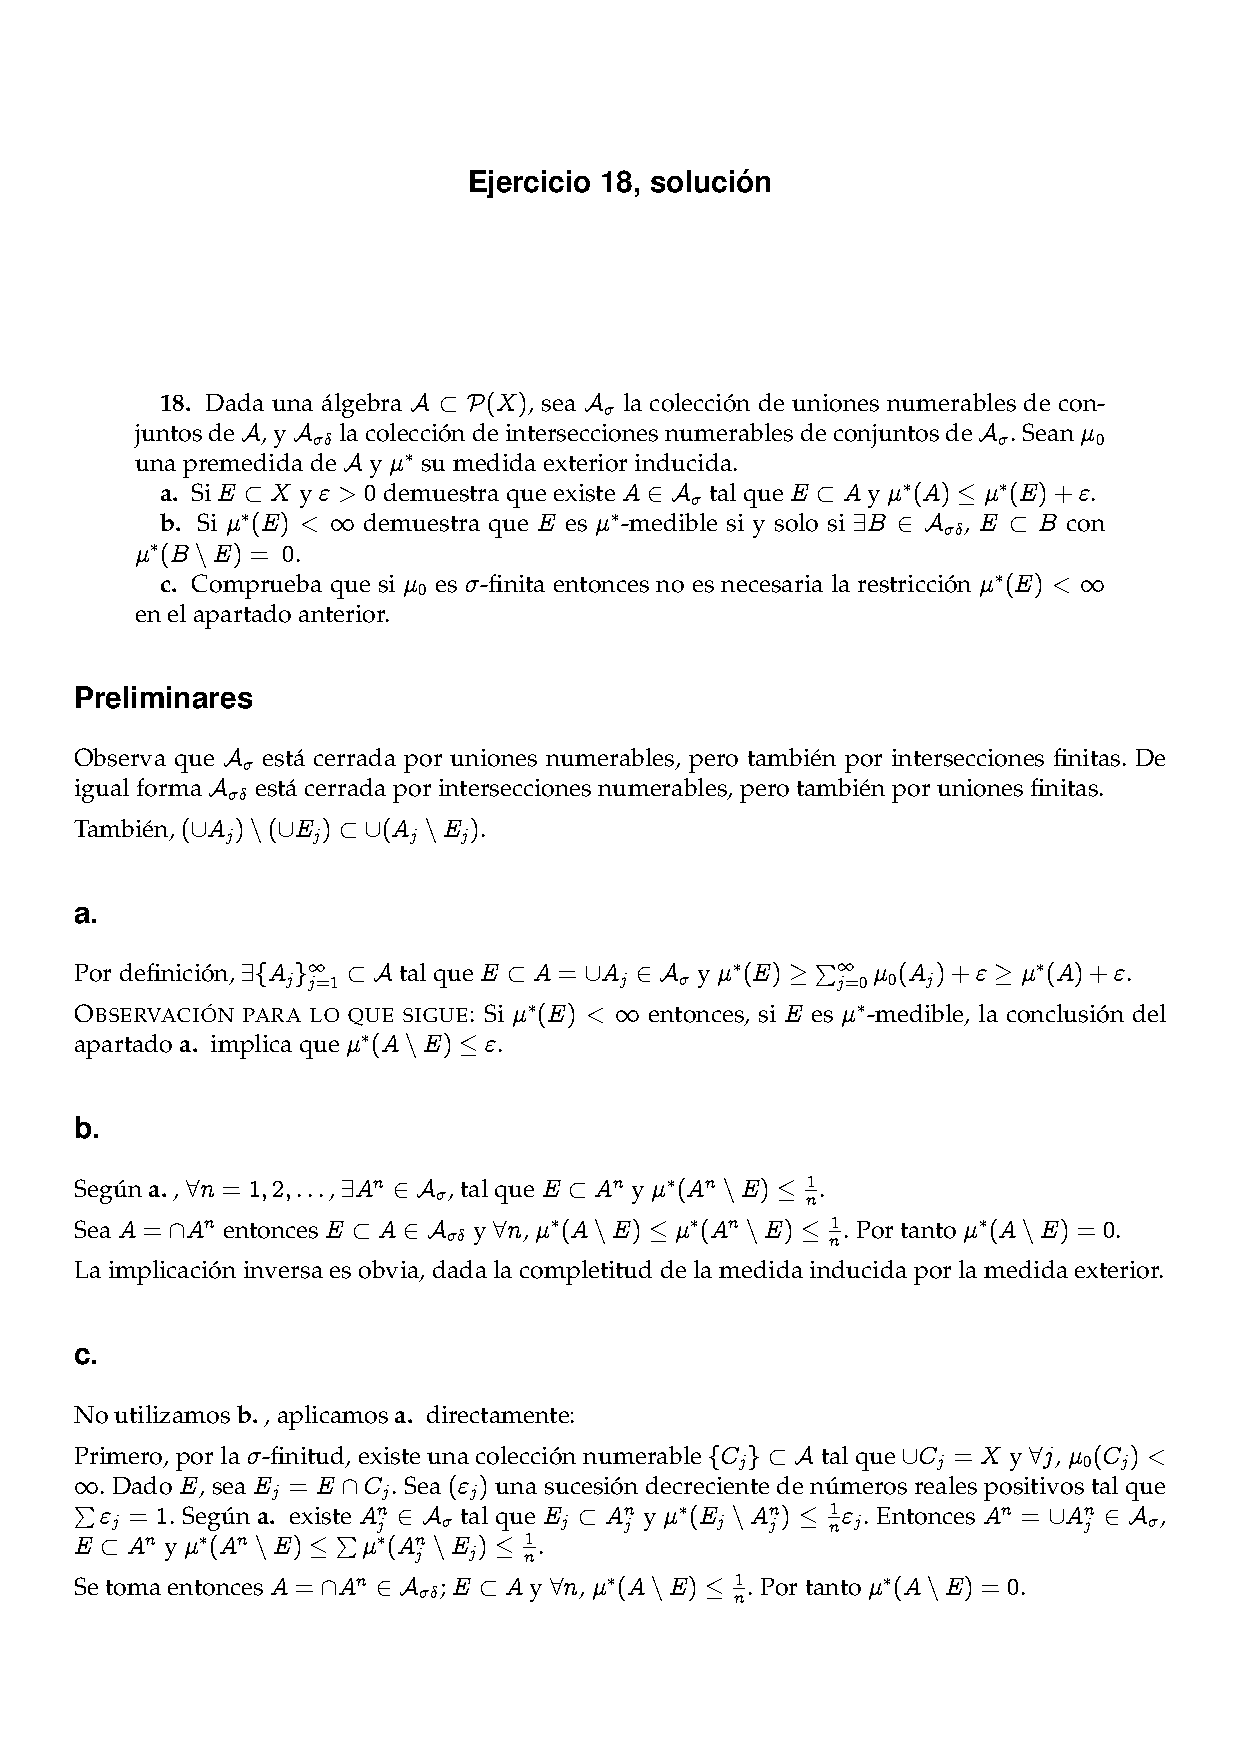
\includepdf[scale=0.9]{pdf/2014-03-18.pdf}
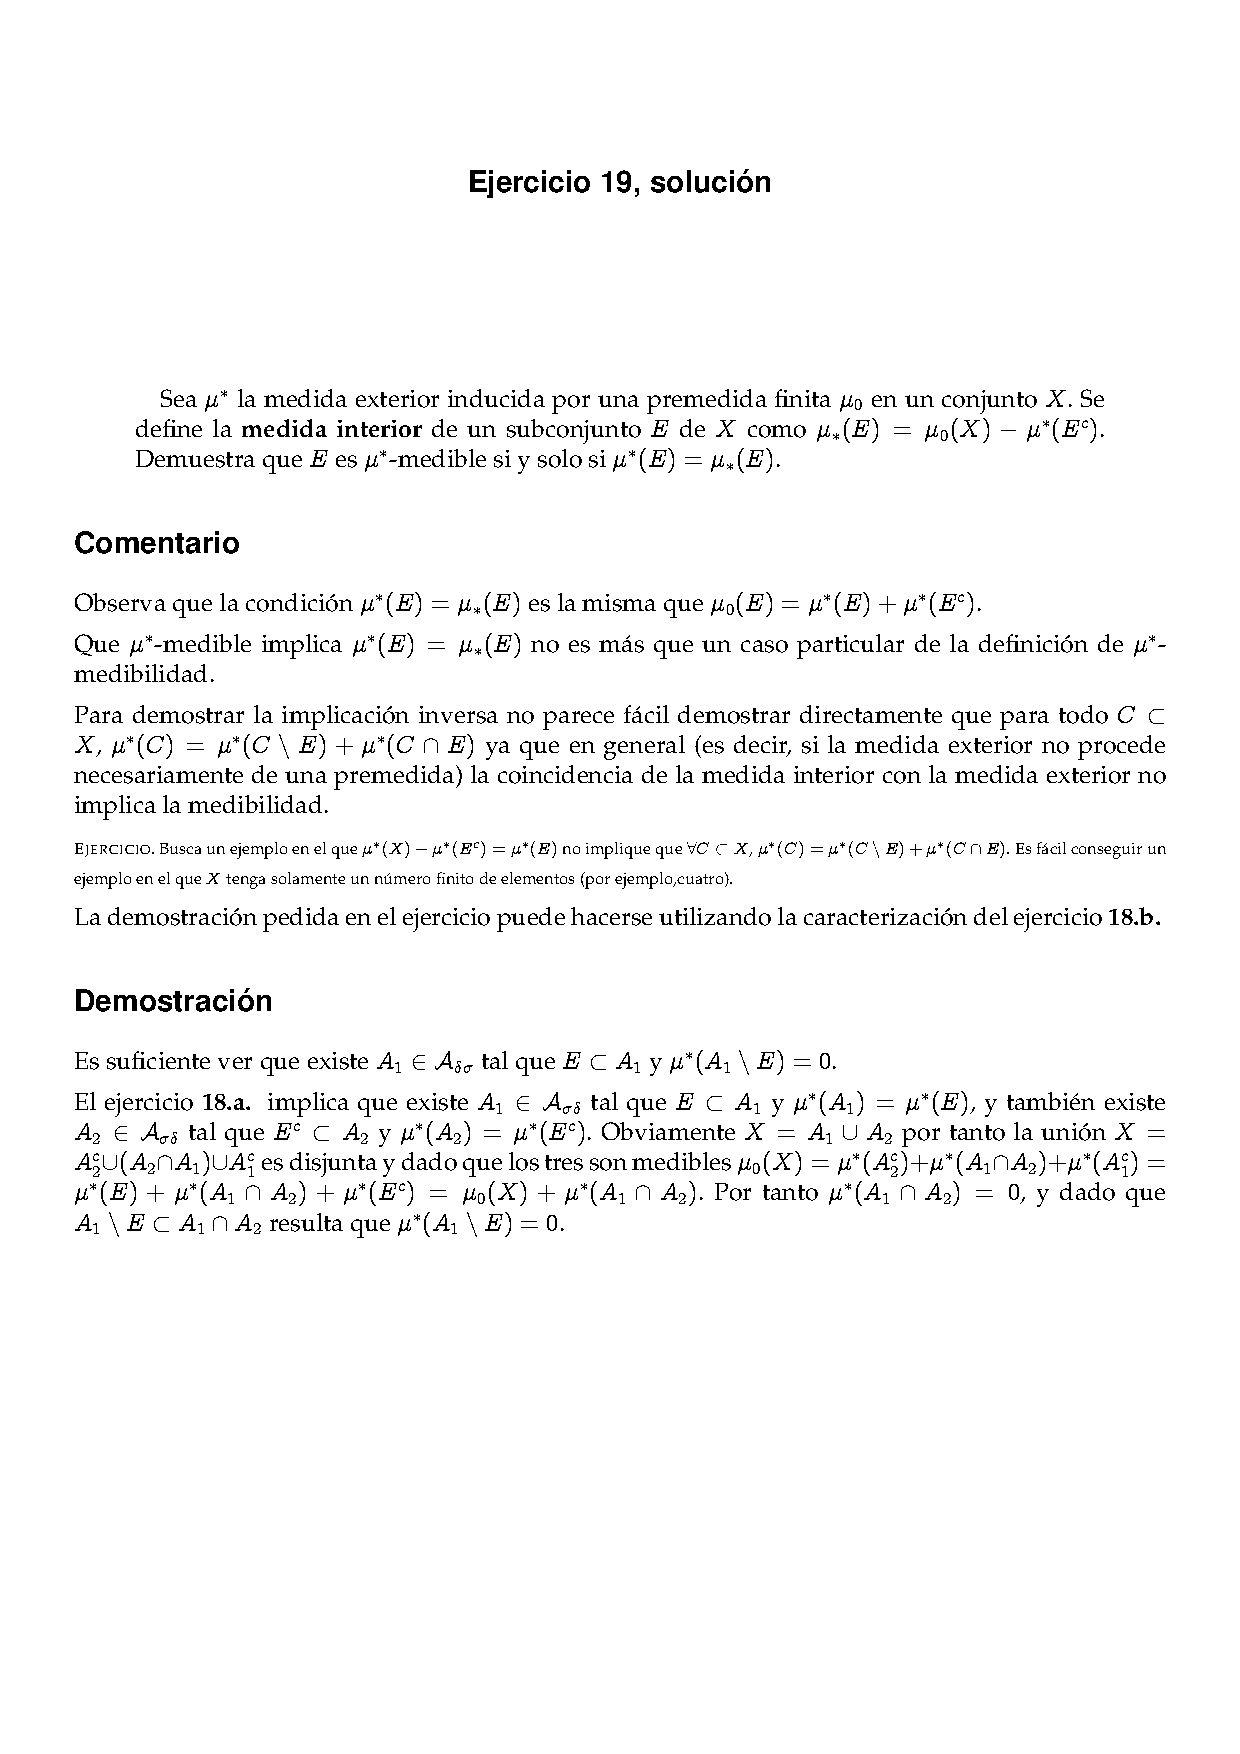
\includepdf[scale=0.9]{pdf/2014-03-19.pdf}
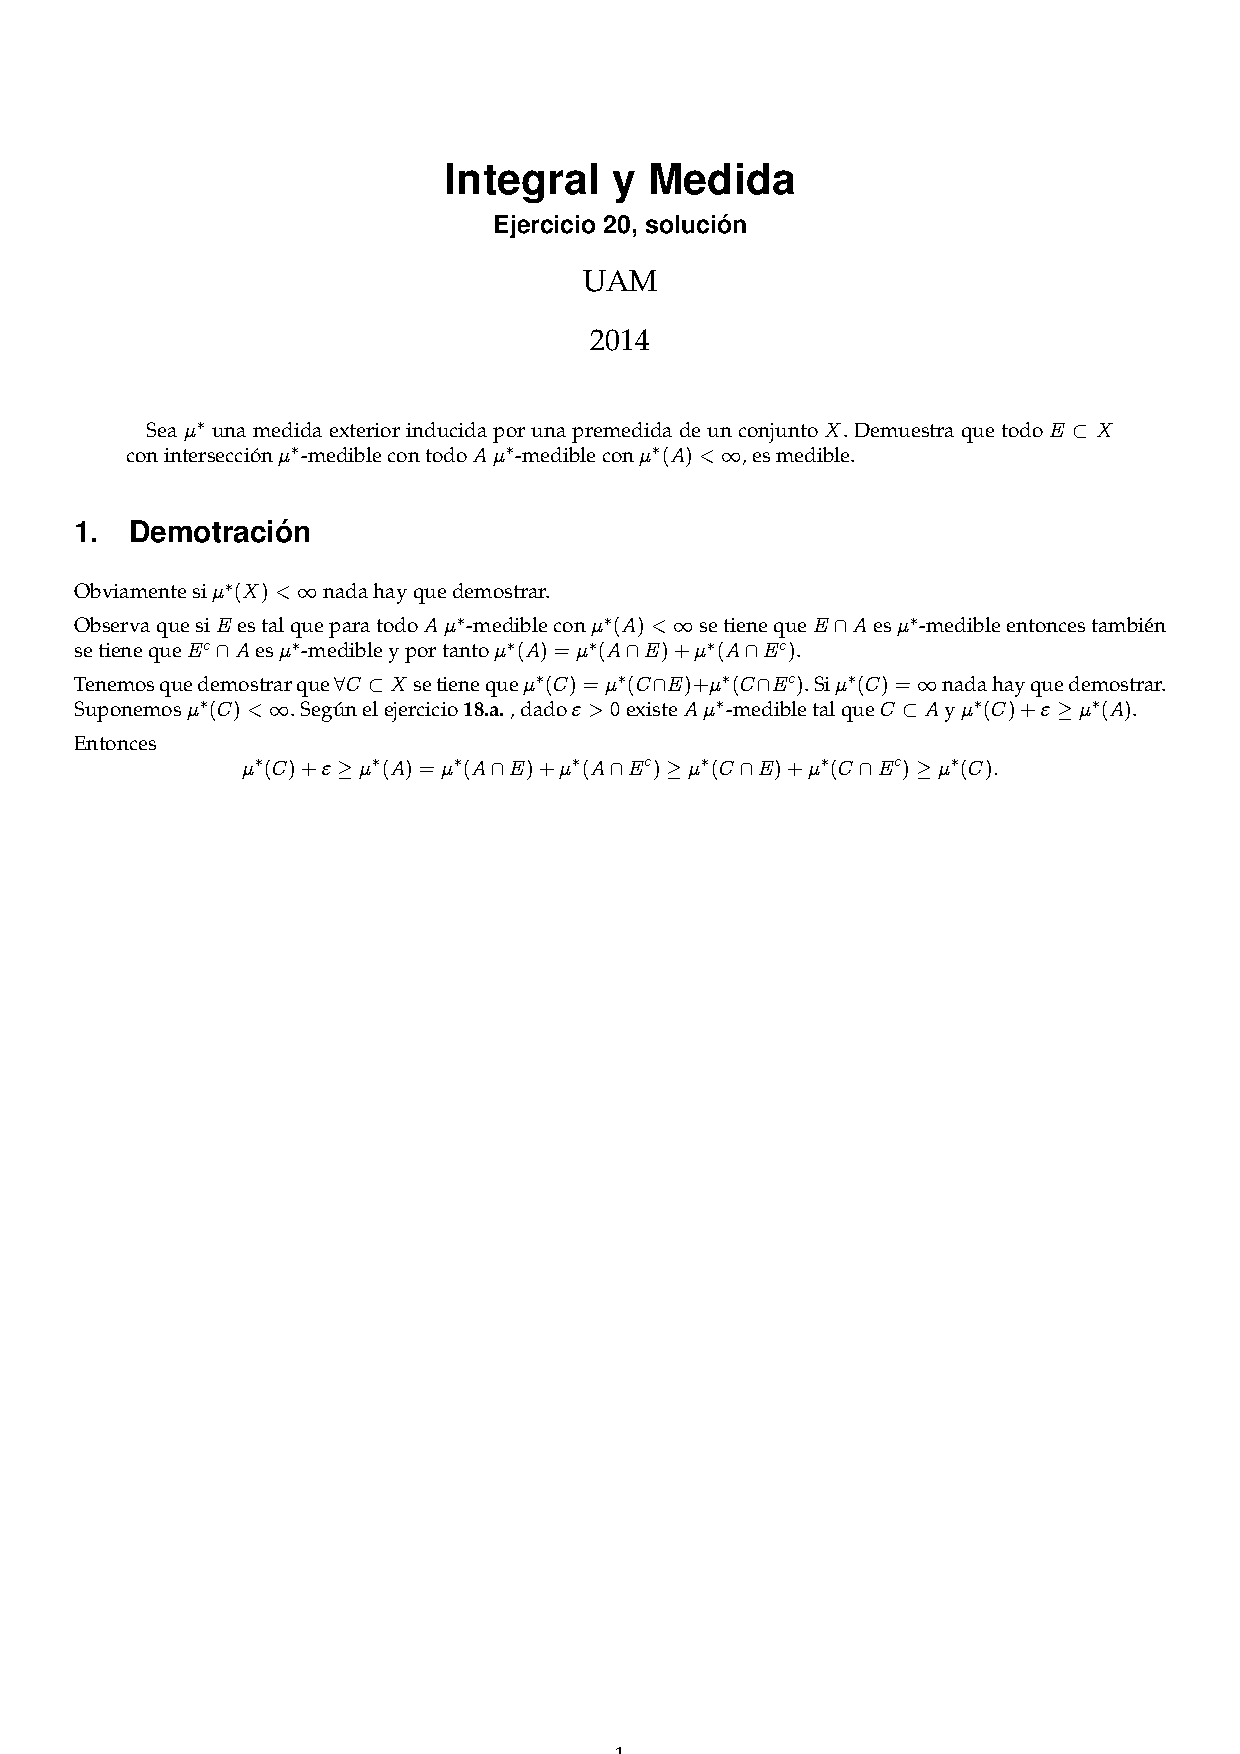
\includepdf[scale=0.9]{pdf/2014-03-20.pdf}

\subsection{Hoja 4}

\begin{problem}
Sea µ la medida de Lebesgue-Stieltjes asociada a la función:
\[F(x)=\left\{ \begin{array}{lcc}
             0 &   si  & x < 1 \\
             \\ x & si & 1 \leq x < 3 \\
             \\ 4 &  si  & 3 \leq x
             \end{array}
   \right.\]

Calcula las siguientes medidas:
\solution
\begin{itemize}
\item $µ(\{1\}) = F(1)-\displaystyle\lim_{x \to 1^-} F(x)$ = 1
\item $µ(\{2\}) = 0$
\item $µ((1, 3]) = F(3)-F(1) = 4 - 1 = 3$
\item $µ((1, 3)) = µ((1, 3]) - µ(\{3\}) = 3 - 1 = 2$
\item $µ([1, 3)) = µ((1, 3)) + µ(\{1\}) = 2 + 1 = 3$
\item $µ([1, 3])) = µ((1, 3]) + µ (\{1\}) = 3 + 1 = 4$
\end{itemize}
\end{problem}

\begin{problem}
Halla funciones de distribución $F$, $F_1$, $F_2$ de forma que, en cada caso, existan $a$ y $b$ tales que:
\begin{enumerate}
\item $µ((a,b)) < F(b)-F(a) < µ([a,b))$, donde $µ=µ_F$
\item $µ_1((a,b)) < µ_1((a,b]) < µ_1([a,b)) < µ_1([a,b])$ y

$µ_2((a,b)) < µ_2([a,b)) < µ_2((a,b]) < µ_2([a,b])$ donde $µ_i = µ_F, \ i=1,2$
\end{enumerate}
\solution
\begin{enumerate}
\item Vale con la función del ejercicio anterior
\item
\textbf{Con i = 1}
\[F_1(x)=\left\{ \begin{array}{lcc}
             0 &   si  & x < 1 \\
             \\ x & si & 1 \leq x < 3 \\
             \\ 3.5 &  si  & 3 \leq x
             \end{array}
   \right.\]

\textbf{Con i = 2}
\[F_2(x)=\left\{ \begin{array}{lcc}
             0 &   si  & x < 1 \\
             \\ x & si & 1 \leq x < 3 \\
             \\ 5 &  si  & 3 \leq x
             \end{array}
   \right.\]
\end{enumerate}

La construcción de estas funciones se ha realizado por la cuenta de la vieja. Si repetimos los cálculos del ejercicio anterior con estas funciones podemos ver que se cumplen las condiciones pedidas (Incluso puede que entendamos de qué va esto)
\end{problem}

\begin{problem}
Sea µ la medida de contar en $(\real, \algbP(\real))$. Para un conjunto finito A $\subset \real$ se define $µ_A(B) = µ(B \cap A)$ para todo $B \subset \real$

\begin{enumerate}
\item Sea $A=\{1,2,...,n,...\}$ ¿Es $µ_A$ una medida de Lebesgue-Stieltjes?. En caso afirmativo halla F tal que $µ_A=µ_F$
\item Sea $A=\{\frac{1}{1},\frac{1}{2},...,\frac{1}{n},...\}$ ¿Es $µ_A$ una medida de Lebesgue-Stieltjes?. En caso afirmativo halla F tal que $µ_A=µ_F$
\end{enumerate}

\solution

\begin{enumerate}
\item Esta medida simplemente cuenta el número de enteros positivos que hay en un conjunto B.

Por tanto, simplemente tenemos que buscar una función que realice esa misma función, por ejemplo:
\[F(x)=\left\{ \begin{array}{lcc}
             0 &   si  & 0 \leq x < 1 \\
             \\ n &  si  & n \leq x < n+1
             \end{array}
   \right.\]

Imitando las cuentas realizadas en el ejercicio 1 podemos que ver:
\begin{itemize}
\item $µ((1,3]))$ = F(3) - F(1) = 2
\item $µ((1,3)) = µ((1,3])) - µ(\{3\}) = 2 - 1 = 1$
\end{itemize}
observamos que, efectivamente, obtenemos el número de enteros de cada intervalo.

\item Esta medida cuenta el número de racionales de la forma $\frac{1}{n}$ que hay en un conjunto.

Esta medida no es de Lebesgue-Stieltjes ya que no puede existir una función F como en el apartado anterior. Esta función debería alcanzar el valor infinito para cualquier intervalo $(0, ε)$, ya que a partir de cierto n todos los siguientes elementos de $A$ se contienen en $(0, ε)$.

%TODO completar esto que creo que no es tan complicado
\end{enumerate}
\end{problem}

\begin{problem}
Sea $F$ la función de distribución
\[F(x)=\left\{ \begin{array}{lcc}
             0 &   si  & x \in (-\infty, -1) \\
             \\ 1+x & si & x \in [-1, 0) \\
             \\ 2+x^2 & si & x \in [0, 2) \\
             \\ 9 &  si  & x \in [2, \infty)
             \end{array}
   \right.\]

Siendo µ=$µ_F$, hallar las siguientes medidas.
\solution
\begin{itemize}
\item $µ(\{2\}) = 3 $
\item $µ([-\frac{1}{2}, 3)) = 9 $
\item $µ((-1,0]\cup (1,2)) 1 + 3 = 4$
\item $µ([0, \frac{1}{2}) \cup (1, 2]) = \frac{1}{4} + 6$
\item $µ(\{x \in \real \tq |x|+2x^2 > 1\})$=$µ((-\infty, -\frac{1}{2})) + µ((\frac{1}{2}, \infty)) = 0 + 9 - 2 - \frac{1}{4} = 7 - \frac{1}{4}$
\end{itemize}
\end{problem}

\begin{problem}
Sea $\appl{f}{\real}{\real}$ no negativa, integrable Riemann sobre cada intervalo finito y tal que $\int_{-\infty}^{\infty}f(x)=1$.

Prueba que $F(x)=\int_{-\infty}^x f(y) dy$ es una función de distribución de probabilidad y que, además, F es continua (f es la función de densidad de F).

Si $f(x)=\ind_{[0,1]}$ hallar $F$

\solution
Simplemente tenemos que ver que F es creciente, continua por la derecha y que se cumple:
\[\lim_{n \to - \infty}F(x)=0 \ \ \lim_{n \to \infty}F(x)=1\]

Observando que $F$ es una integral y que integrar una función equivale a calcular el área encerrada bajo ella, vemos que a medida que avanzamos la x, cada vez estamos calculando un área mayor.

Para ver que es continua por la derecha observamos que:
\[\lim_{h \to 0^+}F(x+h)=\lim_{h \to 0^+} \int_{-\infty}^{\x+h}f(y)dy = \int_{-\infty}^xf(y)dy = F(x)\]
\[\forall x, h \ \lim_{h \to 0^+}\int_{x}^{x+h}f(y)dy=0\]
%TODO completar un poquito más esto que no tengo mucha idea de que está pasando

Suponemos ahora $f(x)=\ind_{[0,1]}$, para responder a la segunda pregunta del enunciado. Entonces
\[F(x)= \int_{-\infty}^{x} \ind_{[0,1]} = \left\{ \begin{array}{lcc}
             0 &   si  & x < 0 \\
             \\ x & si &  0 \leq x \leq 1 \\
             \\ 1 &  si  & 1 \leq x
             \end{array}
   \right.\]
\end{problem}

\begin{problem}
Halla el valor de $k$ para que $f= kx(1-x)\ind_{[0, 1)}$ sea la función de densidad de una medida de probabilidad. Calcula su función de distribución.

\solution
Para que sea función de densidad necesitamos que:
\[\int_{-\infty}^{\infty}f(x) dx = 1\]

Vamos a ver cuánto vale esa integral.
\[\int_{-\infty}^{\infty}f(x) dx = \int_{-\infty}^{\infty}kx(1-x)\ind_{[0, 1)} dx = \int_{-\infty}^{0}kx(1-x)\cdot 0 dx+ \int_{0}^{1}kx(1-x)dx + \int_{1}^{\infty}kx(1-x)\cdot 0 dx = \]
\[= k(\frac{1}{2}-\frac{1}{3})\]
De donde obtenemos fácilmente que $k = \frac{1}{\frac{1}{2}-\frac{1}{3}} = 6$

La función de distribución sería:
\[\F(x)= \int_{-\infty}^{x} \ind_{[0,1]} = \left\{ \begin{array}{lcc}
             0 &   si  & x < 0 \\
             \\ \int_{0}^{x}kt(1-t)dt = (3x^2-2)x^3)& si &  0 \leq x \leq 1 \\
             \\ 1 &  si  & 1 \leq x
             \end{array}
   \right.\]
\end{problem}

\newpage
\begin{problem}
Dado $k$ > 0, sea $f(x)=αe^{-kx}\ind_{[0, \infty)}(x)$
\begin{enumerate}
\item Halla α para que $f$ sea una función de densidad de probabilidad
\item Sea $X$ una variable aleatoria con función de densidad f, si $k=\frac{1}{2}$, calcula la probabilidad de que $X \geq 3$
\item Si $k=\frac{1}{2}$ calcula la probabilidad de que $3 \leq X \leq 6$
\end{enumerate}
\solution
\begin{enumerate}
\item Repitiendo el proceso del ejercicio anterior, debemos hacer que $\int_{0}^{\infty}f(x)dx =1$.

En este caso obtenemos que α=k, es decir, nos encontramos ante una exponencial.

\item
\[\mathbb{P}(X \geq 3) = \int_{³}^{\infty}e^{-kx}dx=e^{\frac{3}{2}}\]

\item Puesto que la función de distribución es continua, la probabilidad de que $X=3$ ó $X=6$ es 0, de modo que podemos calcular la probabilidad pedida como:
\[\mathbb{P}(3 \leq X \leq 6) = \int_{3}^{6}e^{-kx}dx\]
\end{enumerate}
\end{problem}

\begin{problem}
Sea µ la medida de probabilidad definida por la función de distribución:

\[F(x)= \int_{-\infty}^{x} \ind_{[0,1]} = \left\{ \begin{array}{lcc}
             0 &   si  & x \in (- \infty, -1) \\
             \\ \frac{1}{3} & si &  x \in [-1, \sqrt{2}) \\
             \\ \frac{1}{2} + \frac{x-\sqrt{2}}{10} & si &  x \in [\sqrt{2}, 5) \\
             \\ 1 &  si  & x \in [5, \infty)
             \end{array}
   \right.\]

Calcular las siguientes medidas:
\solution

Antes de nada deberíamos comprobar que la función $F(x)$ dada es, efectivamente, una función de distribución. Para ello debemos comprobar que la medida del total es 1 y que se trata de una función creciente.

En este caso nos fiamos y se deja como ejercicio para el lector desconfiado la comprobación de estas propiedades.
\newpage
\begin{enumerate}
\item \[µ((\real \setminus \rac)\cap[\sqrt{2}, 5]) = µ([\sqrt{2}, 5)) = µ((\sqrt{2}, 5]) + µ (\{\sqrt{2}\}) - µ (\{\sqrt{5}\}) =\]
\[ = F(5) - F(\sqrt{2} +(\frac{1}{2}-\frac{1}{3}) -(1-(1-\frac{\sqrt{2}}{10}))=1-\frac{1}{2}+\frac{1}{6}-\frac{\sqrt{2}}{10}\]

\item \[µ((\real \setminus \rac)\cap [-2, \sqrt{2}]) = µ(\{\sqrt{2}\}) = \frac{1}{2}-\frac{1}{3} = \frac{1}{6}\]

\item \[µ(\rac \cap [1,6]) = µ(\{5\}) = \frac{\sqrt{2}}{10}\]
\end{enumerate}

Vamos ahora a por la parte complicada del ejercicio.

\[A_{3n-2} = \left(\frac{2n}{4n+3}, \frac{4n+5}{3n}\right)\]
\[A_{3n} = \left(\frac{4}{5n+2}, \frac{6n+1}{2n}\right)\]
\[A_{3n-1} = \left(-2, \frac{6n-1}{5n+2}\right)\]


Vemos que $\lim A_{3n-2}= [\frac{1}{2}, \frac{4}{3}]$
Vemos que $\lim A_n{3n-1} = (-2, \frac{6}{5})$
Vemos que $\lim A_{3n} = (0^+, 3^+)$

Recordemos que el límite superior de $A_n$ es el conjunto de puntos que están en infinitos conjuntos de la sucesión. Por tanto, todos los puntos contenidos en estos límites se contienen en el límite superior de la sucesión.
\[\limsup A_n = \left(\frac{2n}{4n+3}, \frac{4n+5}{3n}\right) \bigcup  \left(\frac{4}{5n+2}, \frac{6n+1}{2n}\right) \bigcup \left(-2, \frac{6n-1}{5n+2}\right)\]

Por otro lado, el límite inferior es el conjunto de puntos que se encuentran en todos los elementos de la sucesión a partir de uno dado. Así, el límite inferior será la intersección de los límites calculados anteriormente.
\[\liminf A_n = \left(\frac{2n}{4n+3}, \frac{4n+5}{3n}\right) \bigcap  \left(\frac{4}{5n+2}, \frac{6n+1}{2n}\right) \bigcap \left(-2, \frac{6n-1}{5n+2}\right)\]

La parte de calcular la medida de estos límites se deja como ejercicio para el lector
\end{problem}

\begin{problem}
Sea $\appl{F}{\real}{\real}$ una función de distribución
\begin{enumerate}
\item Prueba que el conjunto de puntos de discontinuidad de $F$ es numerable
\item Prueba que el conjunto de puntos de continuidad de $F$ es denso en $\real$
\end{enumerate}
\obs $F$ es monótona luego no tiene más discontinuidades que saltos
\solution
\begin{enumerate}
\item Si tuviésemos una cantidad no numerable de discontinuidades tendríamos un intervalo cerrado que contiene una cantidad no numerable de discontinuidades. Puesto que cada una de esas discontinuidades tenemos un salto, resulta que tendríamos un número no numerable de saltos en un intervalo cerrado.

\end{enumerate}
\end{problem}

\begin{problem}
Variando si es necesario en cada caso el tamaño de los intervalos, construir un conjunto de tipo Cantor cuya medida de Lebesgue sea mayor que 1-ε
\solution
TODO
\end{problem}

\begin{problem}
Sea $µ_F$ la medida de Lebesgue-Stieltjes correspondiente a una función creciente y continua $\appl{F}{\real}{\real}$
\begin{enumerate}
\item Prueba que si A es numerable entonces $µ_F(A)$=0
\item Prueba que existen conjuntos A tales que $µ_F(A)> 0$ y A no contiene ningún intervalo abierto.
\item Si $µ(A)\geq 0$ y $µ(\real \setminus A) = 0$, ¿tiene que ser A denso en $\real$
\end{enumerate}
\obs Se recomienda construir una función $F(x)$ que sea constante en un intervalo
\solution
TODO
\end{problem}

\begin{problem}
Sea $F(x)=log(1 + |x|)\cdot \ind_{[0, \infty)}(x)$
\begin{enumerate}
\item Comprueba que $\appl{F}{\real}{\real}$ es creciente y continua por la derecha.
\item Calcula $µ_F(\{Cantor\})$
\end{enumerate}
\obs El conjunto de Cantor está contenido en $2^n$ intervalos de longitud $\frac{1}{3^n}$
\solution
TODO
\end{problem}

\begin{problem}
Sea µ una medida de Borel en $\real$, finita sobre compactos, con $µ((0, 1])=1$
\begin{enumerate}
\item Prueba que si $\forall s \in \real, µ(s + E)=µ(E)$, entonces µ es la medida de Lebesgue.
\item Prueba que si $\forall s \in \real, µ(rE)=|r|µ(E)$, entonces µ es la medida de Lebesgue
\end{enumerate}
\solution
TODO
\end{problem}

\begin{problem}
Sea m la medida de Lebesgue de $|real$ y $E \subset \real$ medible Lebesgue tal que 0 < m(E) < $\infty$. Demuestra que para todo α, 0<α<1, existe un intervalo abierto I tal que m($I \cap E$) > α m(I)
\solution
TODO
\end{problem}
